\let\negmedspace\undefined
\let\negthickspace\undefined
\documentclass[journal]{IEEEtran}
\usepackage[a5paper, margin=10mm, onecolumn]{geometry}
\usepackage{lmodern} % Ensure lmodern is loaded for pdflatex
\usepackage{tfrupee} % Include tfrupee package

\setlength{\headheight}{1cm} % Set the height of the header box
\setlength{\headsep}{0mm}     % Set the distance between the header box and the top of the text

\usepackage{gvv-book}
\usepackage{gvv}
\usepackage{cite}
\usepackage{amsmath,amssymb,amsfonts,amsthm}
\usepackage{algorithmic}
\usepackage{graphicx}
\usepackage{textcomp}
\usepackage{xcolor}
\usepackage{txfonts}
\usepackage{listings}
\usepackage{enumitem}
\usepackage{mathtools}
\usepackage{gensymb}
\usepackage{comment}
\usepackage[breaklinks=true]{hyperref}
\usepackage{tkz-euclide} 
\usepackage{listings}
\def\inputGnumericTable{}                                 
\usepackage[latin1]{inputenc}                                
\usepackage{color}                                            
\usepackage{array}                                            
\usepackage{longtable}                                       
\usepackage{calc}                                             
\usepackage{multirow}                                         
\usepackage{hhline}                                           
\usepackage{ifthen}                                           
\usepackage{lscape}

\begin{document}

\bibliographystyle{IEEEtran}
\vspace{3cm}

\title{9.7.6}
\author{EE24BTECH11002 - Agamjot Singh}
% \maketitle
% \newpage
% \bigskip
{\let\newpage\relax\maketitle}

\renewcommand{\thefigure}{\theenumi}
\renewcommand{\thetable}{\theenumi}
\setlength{\intextsep}{10pt} % Space between text and floats

\textbf{Question:}
\newline
Solve the differential equation:
\begin{align}
    \frac{dy}{dx} + \sqrt{\frac{1 - y^2}{1 - x^2}} = 0
\end{align}

\textbf{Theoritical solution:}
The given equation is a linear ordinary differential equation.
\begin{align}
    \frac{dy}{dx} &= -\sqrt{\frac{1 - y^2}{1 - x^2}}\\
    \frac{dy}{\sqrt{1 - y^2}} &= -\frac{dx}{\sqrt{1 - x^2}}\\
\end{align}
Integrating on both sides, we get,
\begin{align}
    \int \frac{dy}{\sqrt{1 - y^2}} &= \int -\frac{dx}{\sqrt{1 - x^2}}\\
    \sin^{-1}{y} &= \sin^{-1}{x} + C \text{, where } C \text{ is the constant of integration}
\end{align}

\textbf{Computational Solution:} Euler's method
\newline
By the first principle of derivative,
\begin{align}
    y^{\prime}\brak{x} &= \lim_{h\to0} \frac{y\brak{x + h} - y\brak{x}}{h}\\
    y\brak{x + h} &= y\brak{x} + h\brak{y^{\prime}\brak{x}} \text{, } h\to0
\end{align}
Expressing this system in an iterative format \brak{\text{by method of finite differences}},
\begin{align}
    y\brak{x_{n + 1}} &= y\brak{x_n} + hy^{\prime}\brak{x_n}\\
    y_{n + 1} &= y_n + hy^{\prime}\brak{x_n}\\
    x_{n + 1} &= x_n + h
\end{align}
Substituting the value of $y^{\prime}\brak{x}$, we get,
\begin{align}
    y_{n + 1} &= y_n + h\brak{-\sqrt{\frac{1 - y^2}{1 - x^2}}}
\end{align}
Iteratively plotting the above system taking intial conditions as,
\begin{align}
    x_0 = -0.5 \text{ , } y_{1, 0} = \sin{\brak{1 + \frac{\pi}{6}}}
\end{align}

\begin{figure}[h!]
   \centering
   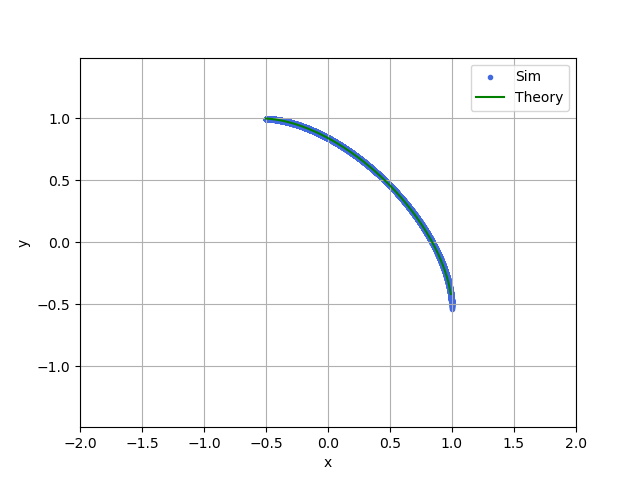
\includegraphics[width=0.7\columnwidth]{figs/graph.png}
    \caption{Computational solution for $y^{\prime} + \sqrt{\frac{1 - y^2}{1 - x^2}} = 0$}
   \label{label}
\end{figure}

\end{document}
